
% Document class: article with font size 11pt
% ---------------
\documentclass[11pt,a4paper]{article}

\setlength{\textwidth}{165mm}
\setlength{\textheight}{240mm}
\setlength{\parindent}{0mm} % S{\aa} meget rykkes ind efter afsnit
\setlength{\parskip}{\baselineskip}
\setlength{\headheight}{0mm}
\setlength{\headsep}{0mm}
\setlength{\hoffset}{-2.5mm}
\setlength{\voffset}{0mm}
\setlength{\footskip}{15mm}
\setlength{\oddsidemargin}{0mm}
\setlength{\topmargin}{0mm}
\setlength{\evensidemargin}{0mm}

\usepackage[a4paper, hmargin={2.8cm, 2.8cm}, vmargin={2.5cm, 2.5cm}]{geometry}
\usepackage[super]{nth}
\PassOptionsToPackage{hyphens}{url}\usepackage{hyperref}
\usepackage{eso-pic} % \AddToShipoutPicture
\usepackage{float} % This will allow precise picture placement, use [H].


% Call packages
% ---------------
\usepackage{comment} %Possible to comment larger sections
%http://get-software.net/macros/latex/contrib/comment/comment.pdf
\usepackage[T1]{fontenc} %oriented to output, that is, what fonts to use for printing characters.
\usepackage[utf8]{inputenc} %allows the user to input accented characters directly from the keyboard

%Support Windows TeXStudio
\usepackage[T1]{fontenc}
\usepackage{lmodern}

%http://mirrors.dotsrc.org/ctan/fonts/fourier-GUT/doc/latex/fourier/fourier-doc-en.pdf
\usepackage[english]{babel}														     % Danish
\usepackage[protrusion=true,expansion=true]{microtype}				                 % Better typography
%http://www.khirevich.com/latex/microtype/
\usepackage{amsmath,amsfonts,amsthm, amssymb}							 % Math packages
\usepackage[pdftex]{graphicx} %puts to pdf and graphic
%http://www.kwasan.kyoto-u.ac.jp/solarb6/usinggraphicx.pdf
\usepackage{xcolor,colortbl}
%http://mirrors.dotsrc.org/ctan/macros/latex/contrib/xcolor/xcolor.pdf
%http://texdoc.net/texmf-dist/doc/latex/colortbl/colortbl.pdf
\usepackage{tikz} %documentation http://www.ctan.org/pkg/pgf
\usepackage{parskip} %http://www.ctan.org/pkg/parskip
%http://tex.stackexchange.com/questions/51722/how-to-properly-code-a-tex-file-or-at-least-avoid-badness-10000
%Never use \\ but instead press "enter" twice. See second website for more info

% MATH -------------------------------------------------------------------
\newcommand{\Real}{\mathbb R}
\newcommand{\Complex}{\mathbb C}
\newcommand{\Field}{\mathbb F}
\newcommand{\RPlus}{[0,\infty)}
%
\newcommand{\norm}[1]{\left\Vert#1\right\Vert}
\newcommand{\essnorm}[1]{\norm{#1}_{\text{\rm\normalshape ess}}}
\newcommand{\abs}[1]{\left\vert#1\right\vert}
\newcommand{\set}[1]{\left\{#1\right\}}
\newcommand{\seq}[1]{\left<#1\right>}
\newcommand{\eps}{\varepsilon}
\newcommand{\To}{\longrightarrow}
\newcommand{\RE}{\operatorname{Re}}
\newcommand{\IM}{\operatorname{Im}}
\newcommand{\Poly}{{\cal{P}}(E)}
\newcommand{\EssD}{{\cal{D}}}
% THEOREMS ----------------------------------------------------------------
\theoremstyle{plain}
\newtheorem{thm}{Theorem}[section]
\newtheorem{cor}[thm]{Corollary}
\newtheorem{lem}[thm]{Lemma}
\newtheorem{prop}[thm]{Proposition}
%
\theoremstyle{definition}
\newtheorem{defn}{Definition}[section]
%
\theoremstyle{remark}
\newtheorem{rem}{Remark}[section]
%
\numberwithin{equation}{section}
\renewcommand{\theequation}{\thesection.\arabic{equation}}


\author{
  \Large{
    Frenzel, Sven Uhrenholdt (\href{mailto:sven@frenzel.dk}{sven@frenzel.dk}) - 130793 - cdn769}\\
}
\title{
  \huge{Compilers\\}
\vspace{3cm}
\Large{\nth{2} Weekly Assignment}
}

\begin{document}

\AddToShipoutPicture*{\put(0,0){\includegraphics*[viewport=0 0 700 600]{include/natbio-farve}}}
\AddToShipoutPicture*{\put(0,602){\includegraphics*[viewport=0 600 700 1600]{include/natbio-farve}}}

\AddToShipoutPicture*{\put(0,0){\includegraphics*{include/nat-en}}}

\clearpage\maketitle
\thispagestyle{empty}

\clearpage\newpage
\thispagestyle{plain}


\section{Task 1}
\begin{enumerate}
	\item[a.)] $\left([og][og]\right)^{+}|\left([og][og][og]\right)^{+}$
	\item[b.)]$\textbf{T} \rightarrow \textbf{R}\ |\ a\textbf{T}b$
	
			  $\textbf{R} \rightarrow c\ |\ c\textbf{R}$
	\item[c).] let-expressions
		\begin{enumerate}
			\item[(i)] As the association of let expressions depends on the content of itself we need to define it for every instance of itself. This is accomplished by \%prec letprec, as it sets the association of the particular instance of the let-expression.
			\item[(ii)] \texttt{\$n} refers to the $n^{th}$ element of the statement. \texttt{\$1} referes to LET, \texttt{\$2} to ID, etc. \texttt{\#m \$n} refers to the $n^{th}$ element in \texttt{\$n}. \texttt{\#1 \$2} thus refers to the first element of ID. Both \texttt{\$} and \texttt{\#} are 1-indexed.
			
			Dec declares something. In this case a declaration with the first element of ID, the first Exp and EQ as the position.
			
			Let is the actual reference to the implementation in the interpreter or intermediate code generator. It passes the declaration into the body and then passes it's body (the second occurrence of Exp) and the position of the let expression (\$1).
		\end{enumerate}	
\end{enumerate}


\section{Task 2}
\begin{enumerate}
	\item[a.)] \texttt{(’a -> bool) -> ’a list -> ’a list}
	\item[b.)] \begin{verbatim}
		CheckExp(exp, vtable, ftable) = case Exp of
		filter(p, arr_exp) =>
		(f, t_0) = GetTypeId (p)
		t_1 = GetTypes (p)
		t_2 = CheckExp (arr_exp, vtable, ftable)
		if (t_1 == t_2 andalso t_0 == Bool)
		then t_1
		else error(); t1
	\end{verbatim}
	\item[c.)] \begin{verbatim}
		CheckExp(exp, vtable, ftable) = case exp of
		filter( Lambda(ret_type, id_type_lst, body), arr_exp ) =>
		t_0 = CheckExp(ret_type, vtable, ftable)
		t_1 = CheckExp(body, vtable, ftable)
		(v, t_2) = id_type_lst
		t_3 = CheckExp (arr_exp, vtable, ftable)
		if (t_1 == t_2 andalso t_2 == t_3 andalso t_0 == Bool)
		then t_1
		else error(); t1
	\end{verbatim}
\end{enumerate}


\section{Task 3}
\begin{figure}[H]
	\centering
	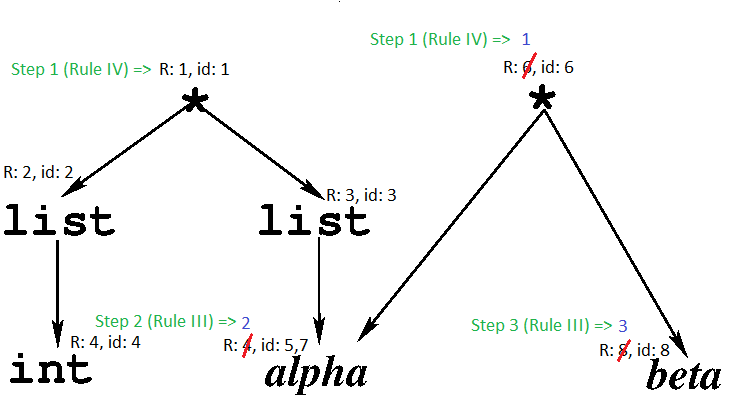
\includegraphics[width=0.5\textwidth]{img/mgu}
	\caption{MGU applied to the given unification graph.}
	\label{fig:mgu}
\end{figure}

$\alpha$ is the type \textit{list(int)}, $\beta$ is the type \textit{list(list(int))} and the unified type is \textit{list(int) * list(list(int))}.


\newpage
\bibliography{mybib}
\bibliographystyle{ieeetr}


\end{document}
